\chapter{Estudio general de la propagación de ondas}
\chaptermark{Ondas}

\begin{miparrafo}
Para la física, una onda (del latín unda) consiste en la propagación de una perturbación de alguna propiedad del espacio, por ejemplo, densidad, presión, campo eléctrico o campo magnético, implicando un transporte de energía sin transporte de materia. El espacio perturbado puede contener materia (aire, agua, etc.) o no (vacío).

La magnitud física cuya perturbación se propaga en el medio se expresa como una función tanto de la posición como del tiempo 

$\psi ({\vec  {r}},t)$. Matemáticamente se dice que dicha función es una onda si verifica la ecuación de ondas:

$$\displaystyle \grad^2 \psi (\vec r ,t)= \pdv[2]{\psi}{t}(\vec r ,t)$$

donde $v$ es la velocidad de propagación de la perturbación. Por ejemplo, ciertas perturbaciones de la presión de un medio, llamadas sonido, verifican la ecuación anterior.

\begin{figure}[H]
		\centering
		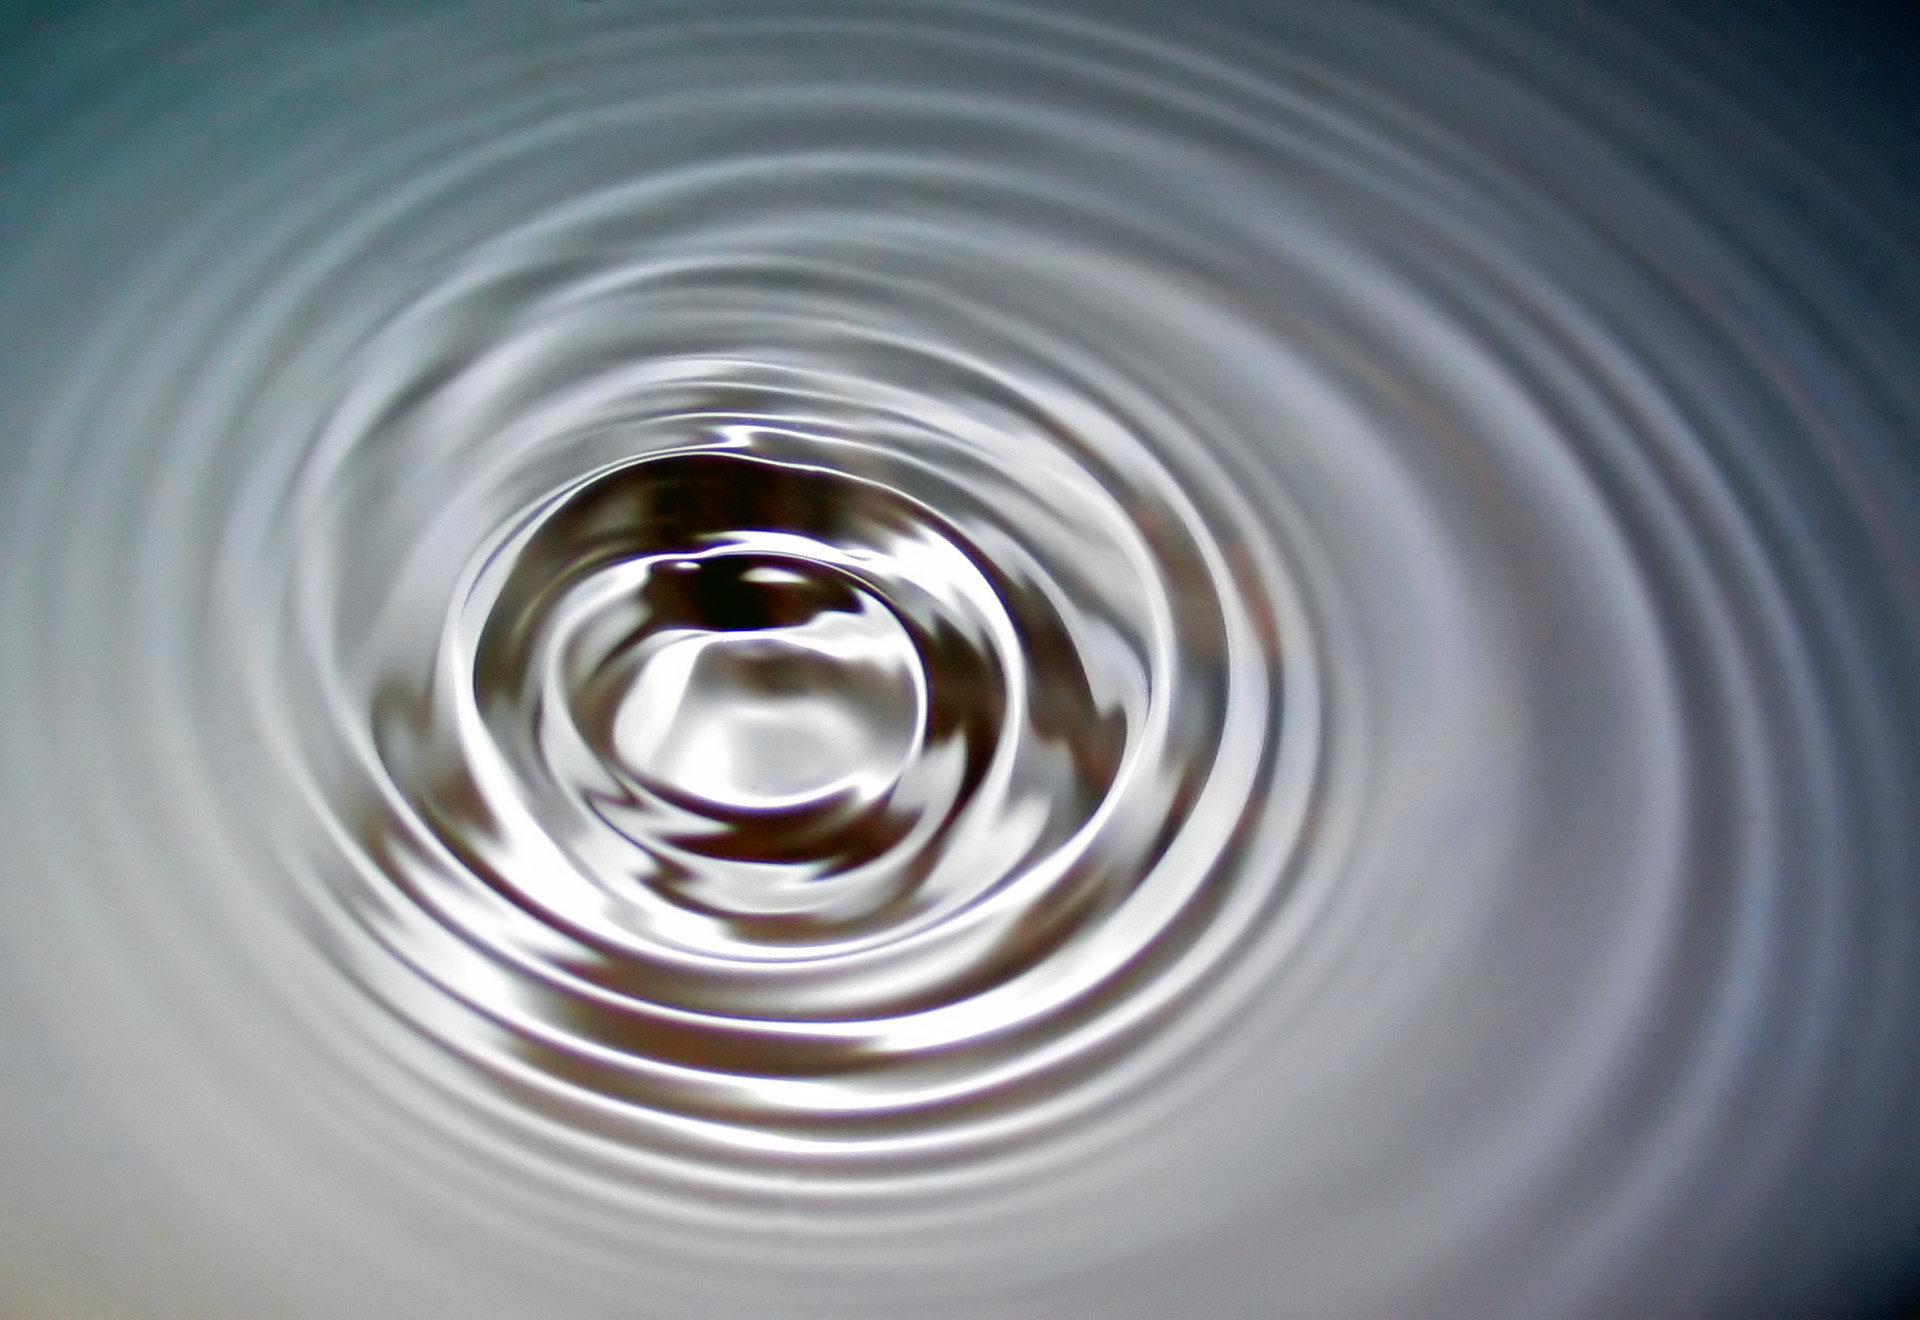
\includegraphics[width=.75\textwidth]{imagenes/imagenes21/T21IM01.png}
	\end{figure}

Las ondas se producen como consecuencia de oscilaciones y vibraciones de la materia, que se propagan en el tiempo según lo descrito por la Teoría de ondas, la rama de la física encargada de comprender dicho fenómeno, sumamente común en el universo.

De acuerdo al origen de las ondas o de la naturaleza del medio a través del cual se propagan, dependerán los efectos de su aparición y sus características. Así, podemos hablar de ondas de luz, de sonido, etc., cada una con propiedades físicas y frecuencias diferentes, dependiendo, entre otras cosas, del medio en el que se propagan y de cuánta energía transportan.

Algunas ondas, como las sonoras, no pueden transportarse en el vacío, requieren de un medio físico. Otras, como las ondas electromagnéticas, pueden hacerlo perfecta y velozmente: es así como operan los satélites artificiales que reenvían información a la Tierra mediante microondas.
\end{miparrafo}

\section[Propagación de una perturbación en una dirección. Ecuación de ondas]{Propagación de una perturbación en una dirección. Ecuación de ondas\sectionmark{Perturbación en una dirección}}
\sectionmark{Perturbación en una dirección}

$\psi$ es una magnitud que existe en un momento en un determinado punto del espacio que lo perturba propagándose en él. Llamemos $v$ a la velocidad con que $\psi$ se transmite. Primera hipótesis, la perturbación  se desplaza a $v_cte$. Incluimos la segunda hipótesis: la magnitud perturbada $\psi$ no sufre amortiguamiento, no se debilita.

 \begin{figure}[H]
		\centering
		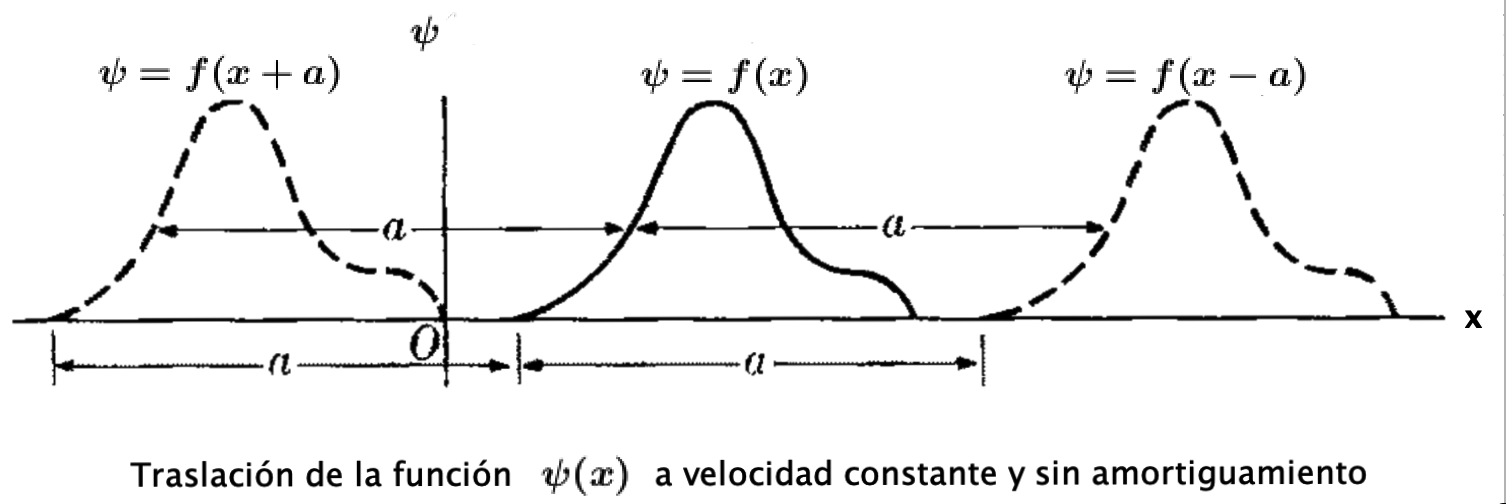
\includegraphics[width=1\textwidth]{imagenes/imagenes21/T21IM02.png}
	\end{figure}
	
Consideramos la curva $\psi(x)=f(x)$ y observamos que $\psi=f(x-a)$ es la misma curva desplazada una distancia $a$ hacia la dereche. Del mismo modo, $\psi=f(x+a)$ es la curva original desplazada $a$ unidades hacia la izquierda.

Si $a=vt$ obtenemos una \emph{curva viajera}. $\psi=f(x-vt)$ es una curva que se mueve a velocidad $v$ hacia la derecha y $\psi=f(x+vt)$ una cueva que se mueve hacia la izquierda.

Concluimos que, en general, $\psi(x,t)\ = f(x \ \pm vt) =\ f \left(t \ \pm \ \dfrac x v \right) $

De otro modo, como $v=cte \to x_2-x_1=v(t_2-t_1) \to $

\begin{equation}
\subrayado{\  \bold{t_2-\dfrac {x_2}v=t_1-\dfrac{x_1}v } \ }	
\end{equation}

Debido a esto, en todas las parejas de puntos espacio-temporales la perturbación tendrá las misma características: $\psi(x,t)=f \left(t-\dfrac x v \right)$.
Si consideramos que la perturbación se desplaza hacia la izquierda, $\psi(x,t)=f \left(t+\dfrac x v \right)$.
La expresión general de como se desplaza en el tiempo una perturbación $\psi$ que se propaga a velocidad constante $v$ y que no se amortigua, en una dirección, lo hace en los dos sentidos, derecha e izquierda, como muestra la siguiente expresión:

\begin{equation}
\subrayado{\  \bold{ \psi(x,t)\ = \ f \left(t \ \pm \ \dfrac x v \right) } \ }	
\end{equation}

 \begin{figure}[H]
		\centering
		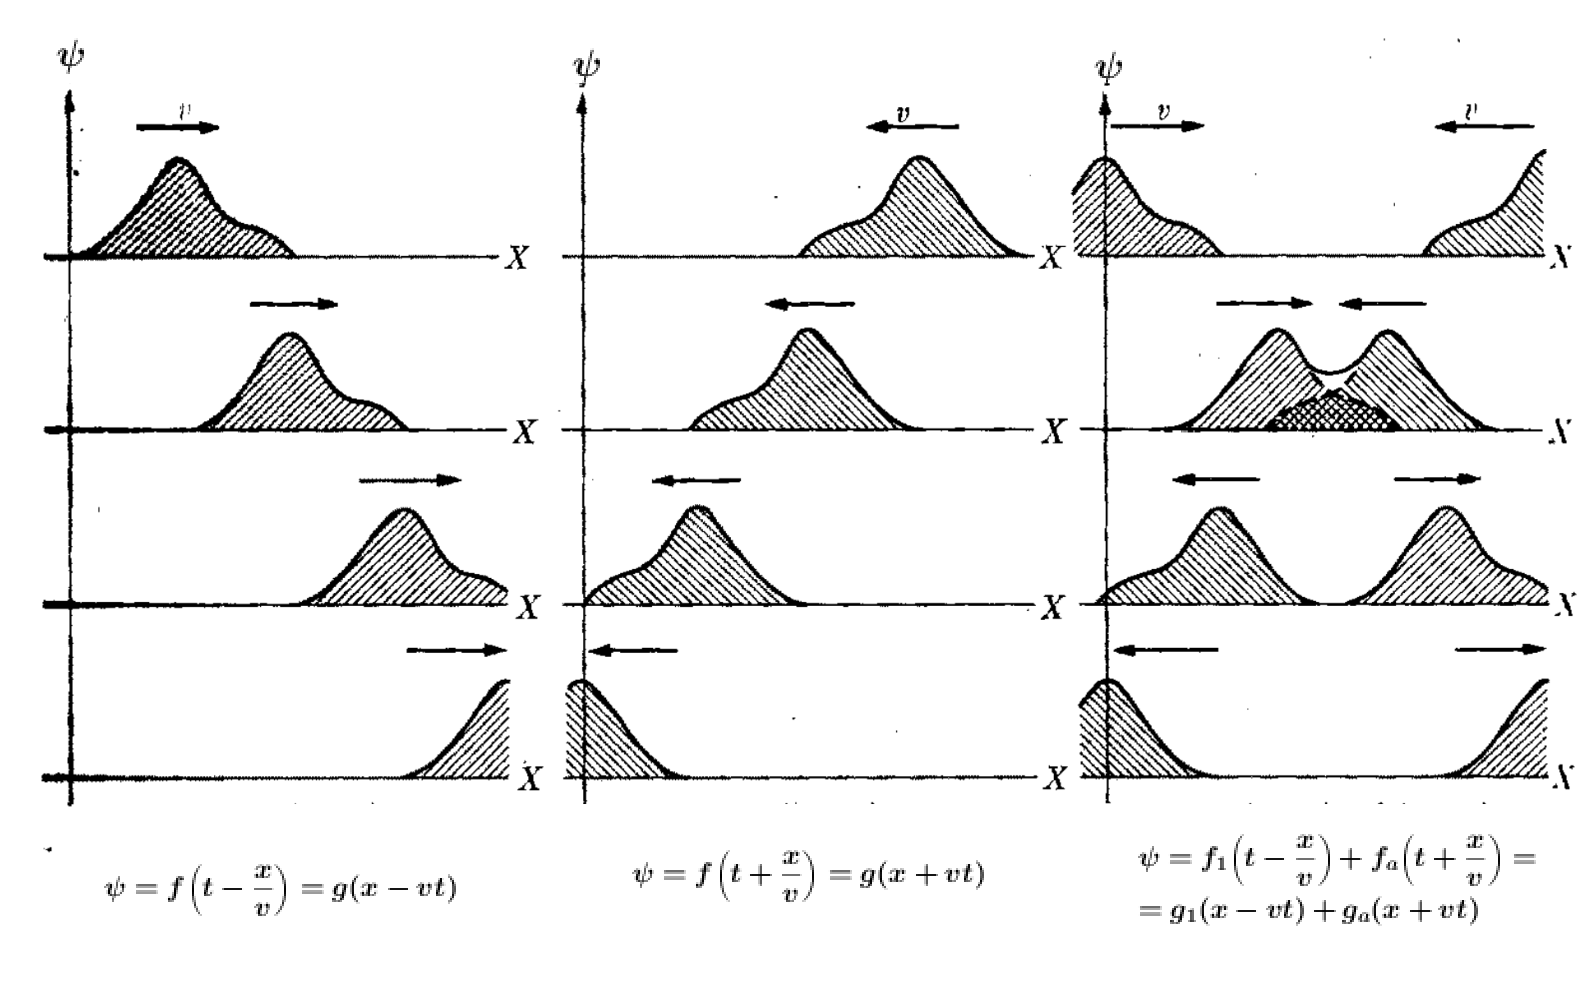
\includegraphics[width=1\textwidth]{imagenes/imagenes21/T21IM03.png}
	\end{figure}

  Veamos si somos capaces de encontrar alguna ecuación diferencial que satisfaga esta relación funcional. Llamamos $\ \boldsymbol{ z=t\pm \dfrac x v }$.
  
 $\displaystyle \pdv{\psi}{t}=\dv{f}{z}\pdv{z}{t}=\dv{f}{z} \ \to  \ \pdv[2]{\psi}{t}=\pdv{t} \dv{f}{t}=\dv[2]{f}{z}\pdv{z}{t}= \dv[2]{f}{z}$
 
 $\displaystyle \pdv{\psi}{x}=\dv{f}{z}\pdv{z}{x} =\pm \dfrac 1 v \dv{f}{z} \ \to \ \pdv[2]{\psi}{x}=\pdv{x} \left[ \pm \dfrac 1 v \dv{f}{z} \right]=\pm \dfrac 1 v \dv[2]{f}{z} \pdv{z}{x}=\dfrac 1 {v^2} \dv[2]{f}{z}$ 
 
 Despejando $\displaystyle \dv[2]{f}{z}$, se encuentra que $\displaystyle \pdv[2]{\psi}{t}=v^2 \pdv[2]{\psi}{x}$, o lo que es lo mismo:
 
\begin{equation}
\label{onda-1D}
\subrayado{ \ \boxed{ \ \boldsymbol{ \pdv[2]{\psi}{x} \ - \ \dfrac 1 {v^2} \ \pdv[2]{\psi}{t}=0 } \ } \ } 	\qquad \textbf{Ec. ondas 1-dim}
\end{equation}

que es una ecuación diferencial de segundo orden con variables independientes. Las soluciones será del tipo $\ \psi=f(t\pm \frac x v)$

La solución más general estará compuesta por una onda que se propaga hacia la derecha y otra hacia la izquierda, $\ \psi=f_1\left( t - \dfrac x v \right) + f_2\left( t + \dfrac x v \right)$

Vamos a ver un caso particular.

\section{Propagación de un fenómeno periódico}

Una gran parte de los fenómenos ondulatorios son de naturaleza periódica.

Tomaremos como origen de distancias el lugar en que se produce la perturbación, $x=0 \to \psi=f(t)$ que suponemos que se repite cada tiempo $T$

Estudiemos cómo se detecta esa perturbación en un punto a una distancia $x$ del origen: $\ t \rightsquigarrow  t-\frac x v: \ \Rightarrow \ \psi=f(t-\frac x v)$

Por el Th\footnote{Th: abreviatura de teorema} de Fourrier, cualquier función periódica se puede expresar como suma de funciones armónicas con un $T$ fundamental y multiplos de éste.

$\psi = a \cos 2\pi \left(\dfrac t T + \varphi \right) \qquad \textcolor{gris}{\omega t = \dfrac {2\pi}T=2\pi \dfrac t T }$

$\text{si }\ \varphi=0 \ \to \ \psi = a \cos 2\pi \dfrac t T $. A una distancia $x$,

$\psi = a \cos 2\pi \left(\dfrac {t-\frac x v}{T}\right)=a\cos 2\pi \left( \dfrac t T - \dfrac{x}{vT} \right)$

Congelando el tiempo y observando como varía la posición (fotografía de la perturbación): 

$\dfrac{2\pi t}{T}-\dfrac{2\pi x}{vT} \ + \ 2\pi = \dfrac{2\pi}{T}-\dfrac{2\pi (x+\lambda)}{vT} \ \to $

\begin{equation}
\subrayado{ \ \boxed{ \ \boldsymbol{\lambda=vT} \ } \ }	\qquad \textbf{longitud de onda}
\end{equation}

Relación del periodo espacial $\lambda$, \emph{longitud de onda}, con el periodo (periodo temporal) $T$

luego:  $\quad \boldsymbol{ \psi = a\cos 2\pi \left( \dfrac t T - \dfrac{x}{\lambda} \right) }$

$\psi$ depende de dos variables, $t \text{ y } x$ y tienen dos periodos, uno temporal $T$ y uno espacial $\lambda$ y una amplitud $a$.

Los puntos en que se verifica $\ 2\pi  \left( \dfrac t T - \dfrac{x}{\lambda} \right) = cte$ son los \emph{puntos equifásicos}. Los puntos equifásicos se desplazan a la misma velocidad que la perturbación $\ v=\dv{x}{t}$

\emph{Puntos en concordancia de fase} son aquellos que, \emph{en un momento determinado}, la diferencia entre sus fases es múltiplo de la longitud de onda $\lambda$. Matemáticamente:

$2\pi \left( \dfrac {\boldsymbol{t}}{T}-\dfrac {x_1}{\lambda}- \right) - 2\pi \left( \dfrac {\boldsymbol{t}}{T}-\dfrac {x_2}{\lambda}- \right) = 2\pi k; \quad \forall k\in \mathbb Z \ \to \ x_1-x_2=k\lambda$

En ese instante  $\boldsymbol{t}$, tenemos que los puntos en concordancia de fase cumplen que $\psi_1=\psi_2$

Llamamos \emph{puntos en oposición de fase} a aquellos puntos en los cuales las diferencias de fase son múltiplos impares de $\pi$; matemáticamente:

$2\pi \left( \dfrac {\boldsymbol{t}}{T}-\dfrac {x_1}{\lambda}- \right) - 2\pi \left( \dfrac {\boldsymbol{t}}{T}-\dfrac {x_2}{\lambda}- \right) =  (2k+1) \pi ; \quad \forall k\in \mathbb Z \ \to \ x_1-x_2=(2k+1) \dfrac \lambda 2$

Para estos puntos, $\ \psi_1=-\psi_2$

\section{Propagación de una perturbación en el espacio}

En una dimensión tenemos: $\quad \displaystyle  \pdv[2]{\psi}{x} \ - \ \dfrac 1 {v^2} \ \pdv[2]{\psi}{t}=0$

generalizando:

\begin{equation}
\displaystyle  \pdv[2]{\psi}{x} \ +  \pdv[2]{\psi}{y} \ + \pdv[2]{\psi}{z} \- \ \dfrac 1 {v^2} \ \pdv[2]{\psi}{t}=0
\end{equation}

Ecuación escalar de ondas en el espacio. (Suponiendo que la magnitud perturbada es una función escalar)

Matemáticamente: $\ \displaystyle \pdv[2]{x}+\pdv[2]{y}+\pdv[2]{z}=\laplacian= \bigtriangleup =\overrightarrow{\grad} \cdot \overrightarrow{\grad}$, es el llamado \textbf{operador ``laplaciana''}.

Si lo que se propaga es una magnitud escalar, $\psi$, la ecuación de ondas en el espacio es:

\begin{equation}
\subrayado{ \ \boxed{ \ \boldsymbol{\laplacian \psi \ - \dfrac 1 {v^2} \ \pdv[2]{\psi}{t}} \ } \ } \quad \textbf{ecuación escalar de ondas 3-D}
\end{equation}

Para una magnitud vectorial que se propague: $\ \vec \psi=\vec i \ \psi_x + \vec j \ \psi_y + \vec k \psi_z\ $ habrá una ecuación escalar por cada componente.

$\displaystyle 
\laplacian \psi_x \ - \dfrac 1 {v^2} \ \pdv[2]{\psi_x}{t}=0; \quad
\laplacian \psi_y \ - \dfrac 1 {v^2} \ \pdv[2]{\psi_y}{t}=0; \quad
\laplacian \psi_z \ - \dfrac 1 {v^2} \ \pdv[2]{\psi_z}{t}=0$

que también podemos escribir vectorialmente como:

\begin{equation}
\label{onda-3D}
\subrayado{ \ \boxed{ \ \boldsymbol{\laplacian \overrightarrow{\psi} \ - \dfrac 1 {v^2} \ \pdv[2]{\overrightarrow{\psi}}{t}} \ } \ } \quad \textbf{ecuación vectorial de ondas 3-D}
\end{equation}

Veamos un caso particular.

\section[Ondas esféricas en un medio homogéneo e isótropo]{Ondas esféricas en un medio homogéneo e isótropo\sectionmark{Ondas esféricas}}
\sectionmark{Ondas esféricas}

Como hipótesis, consideramos el espacio \emph{homogéneo} (igual en todas las partes) e \emph{isótropo} (las propiedades del espacio son independientes de la dirección en que se midan). Por ello, todos los puntos situados en la esfera de radio $r$ trazada desde el centro donde se origina la perturbación estarán en la misma fase, vibrarán del mismo modo.

Consideremos que la magnitud que se propaga es de tipo escalar (sonido de un grito). Veamos como es su ecuación de propagación.

$\psi=f(x,y,z,t)=f(r,t) \ $ (homogeneidad e isotropía). \textcolor{gris}{$\quad (r=\sqrt{x^2+y^2+z^2})$}

$\displaystyle \pdv[2]{\psi}{x}=
\pdv{x} \pdv{\psi}{x}=
\pdv{x} \left( \boldsymbol{\pdv{\psi}{r} \pdv{r}{x}} \right) =
 \pdv{x} \left( \boldsymbol{\dfrac x r \pdv{\psi}{r}}  \right)=$
 
 $\displaystyle
 = \dfrac 1 r \pdv{\psi}{r}+x\pdv{1/r}{x}\pdv{\psi}{r}+x \dfrac 1 r \pdv{x} \pdv{\psi}{r}=
 \dfrac 1 r \pdv{\psi}{r} - \dfrac{x^2}{r^3}\pdv{\psi}{r} + \dfrac{x^2}{r^3}\pdv[2]{\psi}{r}= $
 
 $\displaystyle
 =\dfrac{r^2-x^2}{r^3}\pdv{\psi}{r} + \dfrac{x^2}{r^2} \pdv[2]{\psi}{r}\qquad$ Análogamente para las otras componentes.

 En total tendremos: 
 $\ \displaystyle \laplacian \psi= \pdv[2]{\psi}{x}+ \pdv[2]{\psi}{y}+ \pdv[2]{\psi}{z}=  \pdv[2]{\psi}{r} + \dfrac 2 r \pdv{\psi}{r}$
 
 Por lo que la ecuación de la perturbación 3-D en espacios homogéneso e isótropos (ec. \ref{onda-3D}) queda como:
 
 \begin{equation}
 \laplacian \psi \ = \ \pdv[2]{\psi}{r} \ + \ \dfrac 2 r \ \pdv{\psi}{r} \ - \ \dfrac 1 {v^2} \ \pdv[2]{\psi}{t} \ = \ 0 	
 \end{equation}

Si multiplicamos esta ecuación por $r$: $\quad \displaystyle r\  \pdv[2]{\psi}{r}  +   2  \ \pdv{\psi}{r}  -  \dfrac r{v^2}\  \pdv[2]{\psi}{t} = 0$ 

O, lo que es lo mismo, $\quad \displaystyle \pdv[2]{\psi r}{r}-\dfrac 1 {v^2} \pdv[2]{\psi r}{t}=0$, ya que $r$ no depende de $t$.

Llamando $\quad \boldsymbol{\Psi=\psi r}$, podemos escribir:

\begin{equation} 
\subrayado{ \ \boldsymbol{\pdv[2]{\Psi}{r}\ -\ \dfrac 1 {v^2} \ \pdv[2] {\Psi}{t}=0}\ }
\end{equation}

Ecuación que coincide con la forma de la ecuación (\ref{onda-1D}) de propagación de una perturbación en una dimensión, por lo que el resultado debe ser como el de una dimensión:

$\Psi= r \psi = f_1(\left( t-\dfrac r v \right)+f_2(\left( t+\dfrac r v \right) \ \to \ \psi = \dfrac 1 r f_1(\left( t-\dfrac r v \right)+ \dfrac 1 r f_2(\left( t-\dfrac r v \right)$

Como solución particular escribiremos la de una perturbación periódica por el desarrollo de Fourrier, para una perturbación desplazándose en las $x$ positivas:

\begin{equation}
\boldsymbol{ \psi= \dfrac a r \cos 2\pi \left( \dfrac t T - \dfrac r v  \right)	}
\end{equation}

En espacio homogéneo e isótropo la perturbación. se caracteriza porque la amplitud se debilita de modo inversamente proporcional a la distancia $r$.

Se suelen definir las \emph{superficies equifases} o \emph{superficies de onda} como aquellas superficies que en todo instante tienen la misma fase. En el caso de propagación en espacios homogéneos e isótropos, las superficies de onda son esféricas.

También se habla de puntos en concordancia y en oposición de fase como aquellas superficies esféricas cuyas diferencias son múltiplos de $2\pi$ o de $(2k+1)\pi$, respectivamente: $r_2-r_1=k\lambda$ o $r_2-r_1=(2k+1)\lambda/2$

Se define la \emph{dirección de propagación de onda} en un punto dado como la dirección de la normal a la superficie de onda que pase por ese punto.

Veamos ahora como se propaga una onda vectorial en el espacio, supuesto éste homogéneo e isótropo. $\vec \psi=\psi \vec u$

La solución más general es $ \psi=\dfrac v{r^2} f(\left( t-\dfrac r v \right) + \dfrac 1 r f'(\left( t-\dfrac r v \right)$, 

con $f'$ derivada temporal de $f$. Como caso particular consideramos una perturbación periódica que desarrollada por Fourrier como movimientos armónicos podemos escribir:

$\psi  = \dfrac v{r^2} A sin 2\pi \left( \dfrac t T - \dfrac r \lambda \right)+\dfrac 1 r \dfrac {2\pi}{T} A \cos 2 \pi \left( \dfrac t T - \dfrac r \lambda \right)$

Como el primer término varía con el inverso de la distancia al cuadrado será despreciable frente al segundo término para distancias grandes y llamando $\ a=\dfrac{2\pi}{T} A$, tendremos:

\begin{equation}
\label{ondas-esfericas-grandes-distancias}
\boldsymbol{ r>>1 \ \to \  \psi \ \approx \ \dfrac a r \cos 2\pi \left( \dfrac t T - \dfrac r \lambda \right) }
\end{equation}

que coincide con el comportamiento de una onda escalar a una distancia $r$.
\vspace{10mm}  %**********************************************
\section{Ondas planas}

La onda plana asociada a la propagación de una magnitud escalar se caracteriza por que, en un instante determinado, la magnitud $\vec \psi$ es la misma en cada uno de los puntos de los planos perpendiculares  a una dirección dada (dirección de propagación). Las superficies de onda serán planos geométricos perpendiculares a la dirección de propagación de la onda.
	\begin{figure}[H]
		\centering
		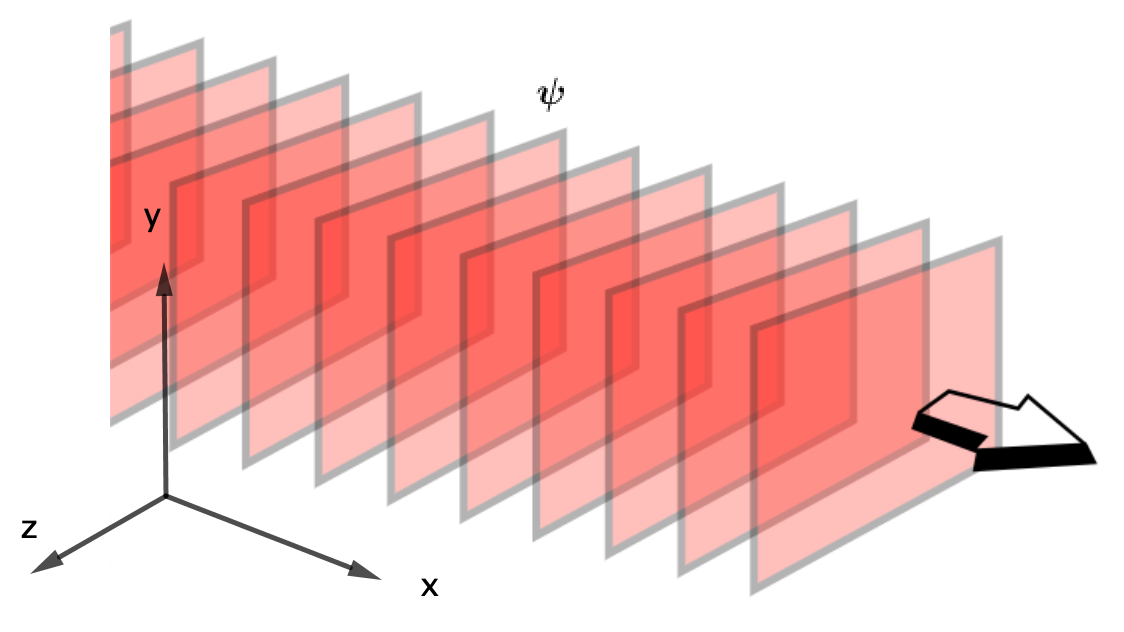
\includegraphics[width=.8\textwidth]{imagenes/imagenes21/T21IM04.png}
	\end{figure}
\vspace{40mm}  %**********************************************
Elegimos $x$ como eje de propagación de la onda. Las superficies de onda son planos $YZ\ \bot \ \overrightarrow{\mathcal OX}$.

Por definición de onda plana: $\ \displaystyle \pdv{\vec \psi}{y}=\pdv{\vec \psi}{z}=0;\ \pdv{\vec \psi}{x}\neq 0$

La ecuación de ondas, para esta onda plana, se escribe como:

\begin{table}[H]
\begin{tabular}{ccc}
$\displaystyle \pdv[2]{\psi_x}{x}-\dfrac 1 v^2\ \pdv[2]{\psi_x}{t}=0\quad $ &$ \ \to \ $&$\displaystyle \quad \psi_x=a_x\ \cos 2 \pi \left( \dfrac t T - \dfrac x \lambda \right)$  \\
$\displaystyle \pdv[2]{\psi_y}{y}-\dfrac 1 v^2\ \pdv[2]{\psi_y}{t}=0\quad $ &$ \ \to \ $&$\displaystyle \quad \psi_y=a_y\ \cos 2 \pi  \left( \dfrac t T - \dfrac x \lambda \right)$  \\
$\displaystyle \pdv[2]{\psi_z}{z}-\dfrac 1 v^2\ \pdv[2]{\psi_z}{t}=0\quad $ &$ \ \to \ $&$\displaystyle \quad \psi_z=a_z\ \cos 2 \pi  \left( \dfrac t T - \dfrac x \lambda \right)$  
\end{tabular}
\end{table}

Estas ecuaciones son formalmente análogas a las de la propagación de una perturbación en una dirección.

$$\boldsymbol{\psi\ =\ \sqrt{\psi_x^2+\psi_y^2+\psi_z^2}\ =\ a \cos 2 \pi \left( \dfrac t T - \dfrac x \lambda \right) }$$

donde $ \ a=\sqrt{a_x^2+a_y^2+a_z^2}$

Comparando esta ecuación co la dela ondas esféricas a grandes distancias del cuerpo emisor, ec \ref{ondas-esfericas-grandes-distancias}, observamos que estas son similares a ondas planas. (Rayos que parten del sol y llegan a la superficie terrestre).

\begin{figure}[H]
		\centering
		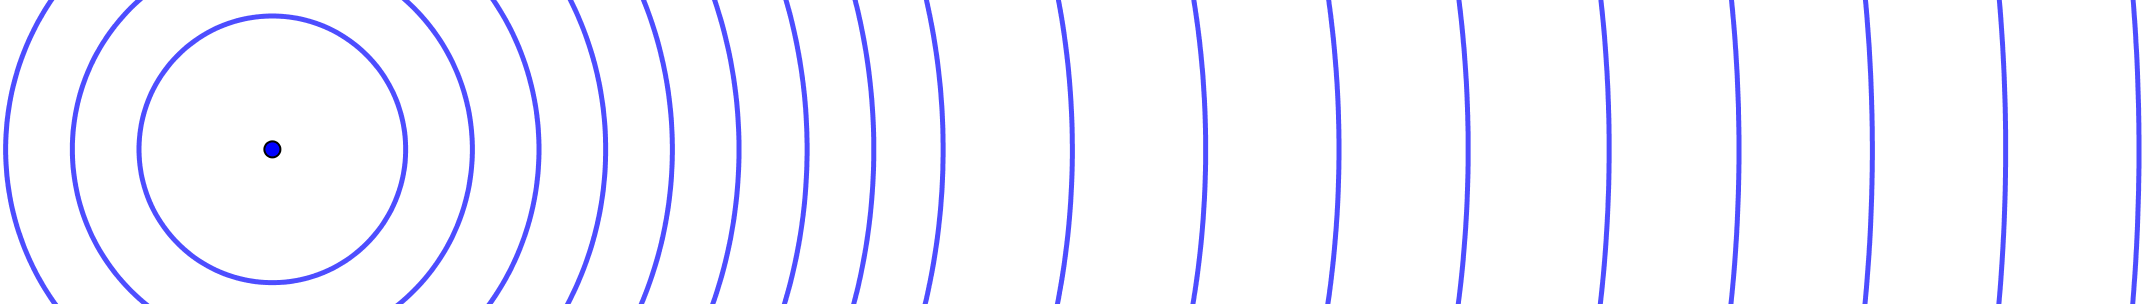
\includegraphics[width=.75\textwidth]{imagenes/imagenes21/T21IM05.png}
	\end{figure}

Cuando se habla de ondas vectoriales, se suele distinguir entre \emph{ondas transversales} y \emph{ondas longitudinales}.

Una \emph{onda es transversal} cuando el vector asociado a la magnitud que se propaga vibra perpendicularmente a la dirección de propagación.

Una \emph{onda es longitudinal} cuando el vector asociado a la magnitud que se propaga vibra en la dirección de propagación.

\begin{figure}[H]
		\centering
		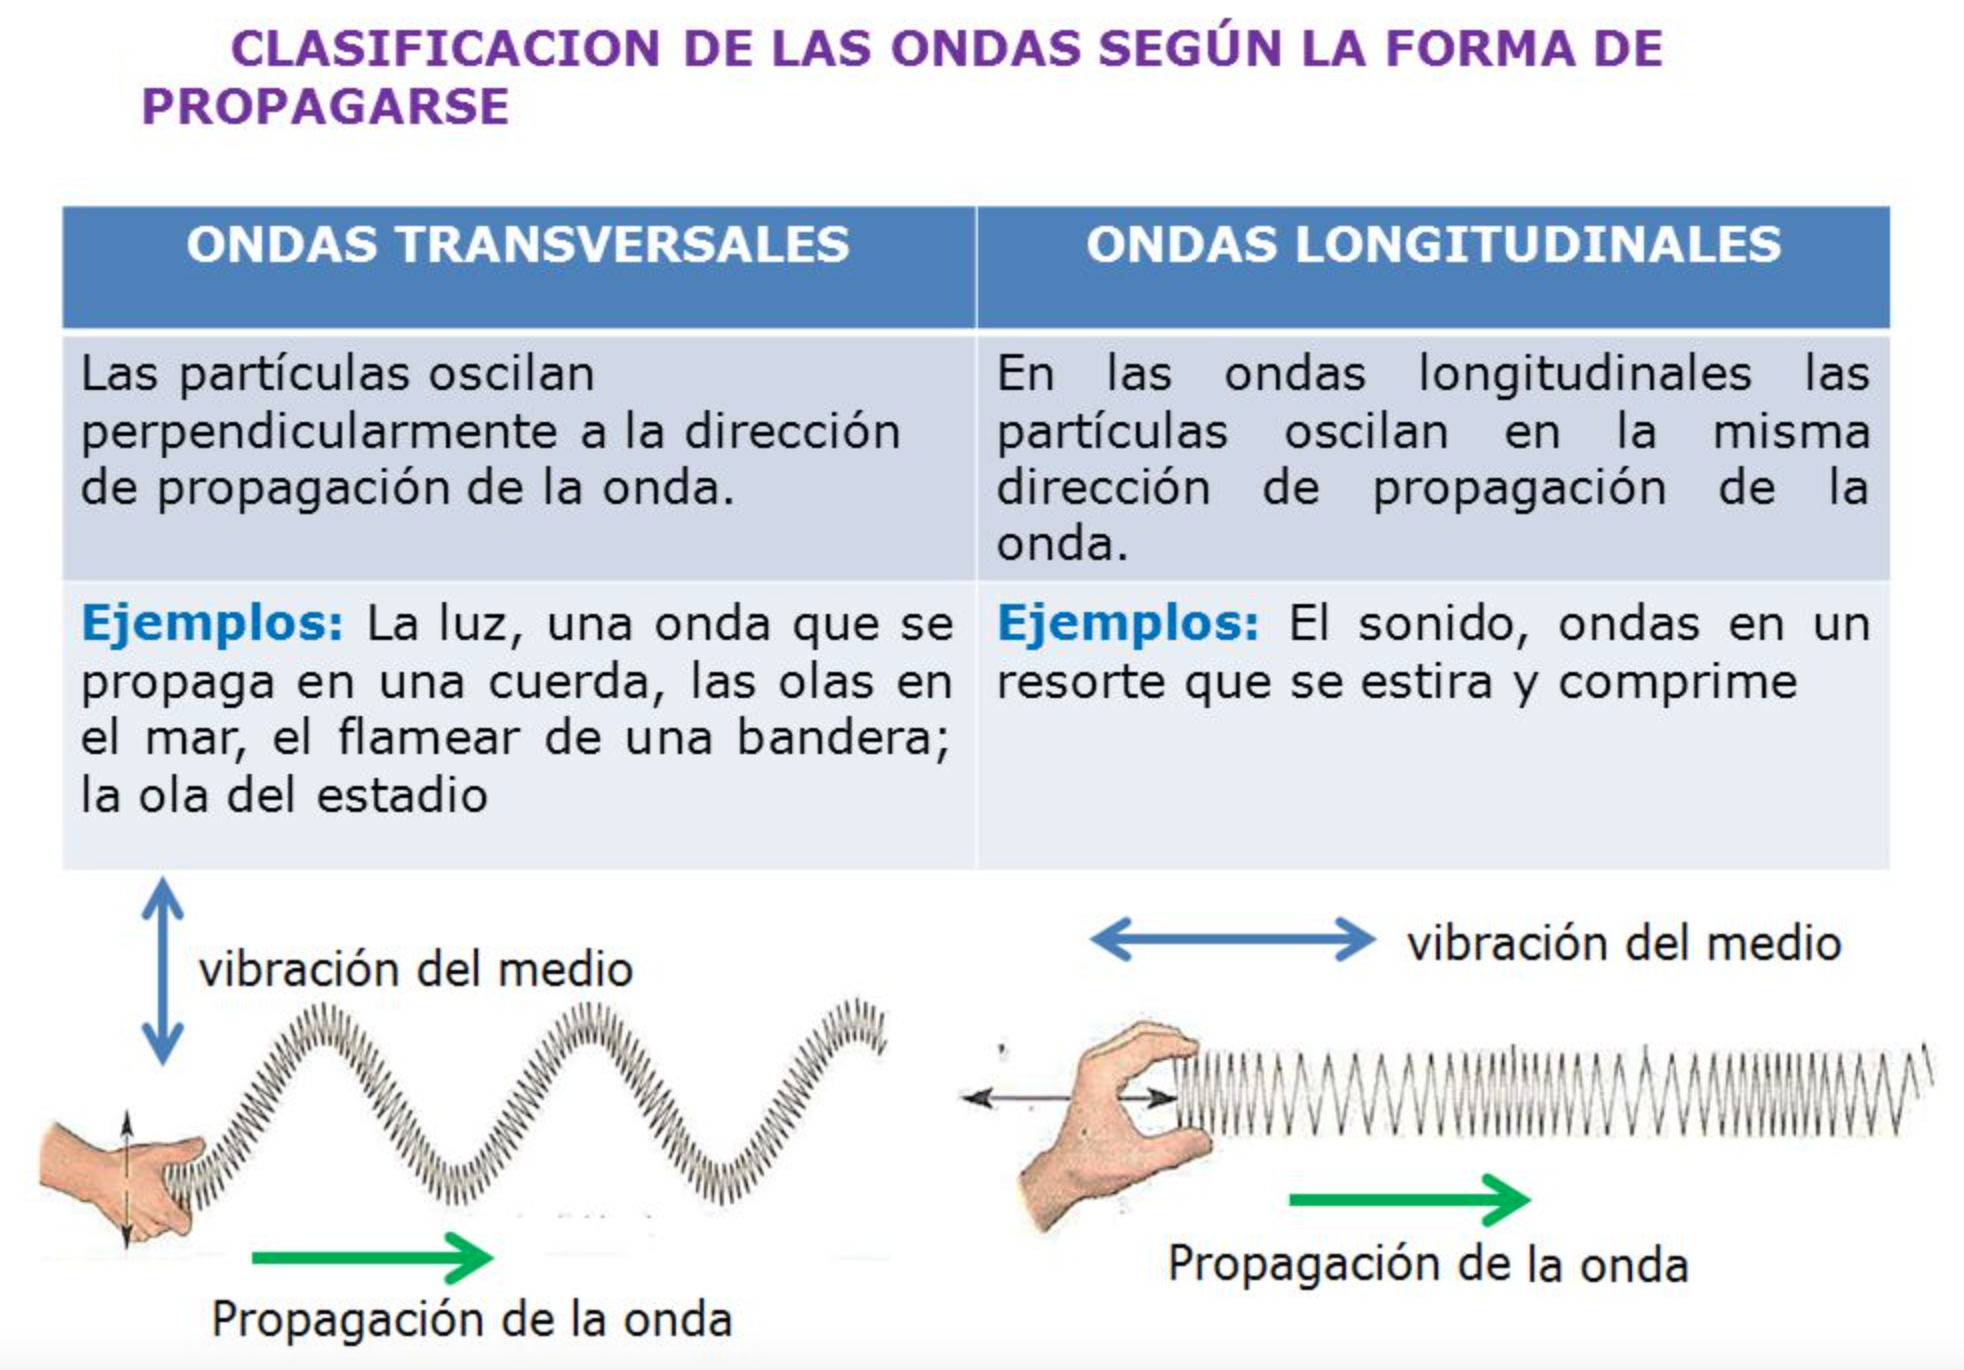
\includegraphics[width=.9\textwidth]{imagenes/imagenes21/T21IM06.png}
	\end{figure}
	

\section{Problemas}
\vspace{10mm} %***************************************
\begin{prob}
Un resorte tiene una constante $k$ y una masa $m$ cuelga de él. Se corta el resorte por la mitad y la misma masa de cuelga de una de las dos mitades. ¿La frecuencia de la vibración es la misma, mayor o menor antes y después de cortar el resorte.	
\end{prob}

\begin{multicols}{2}
$mg=-k_1x;\quad mg=-k_2x/2$

$k_1/k_2=1/2$

$\omega=\sqrt{k m}$

$\dfrac {\omega_1}{\omega_2}=\sqrt{\dfrac 1 2}$

$\omega_2=\sqrt{2}\ \omega_1$
\begin{figure}[H]
		\centering
		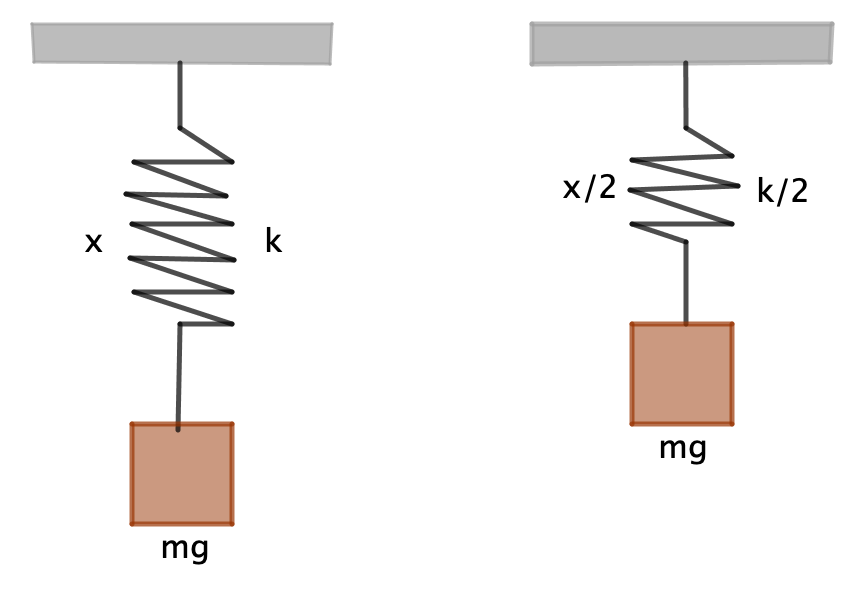
\includegraphics[width=.4\textwidth]{imagenes/imagenes21/T21IM07.png}
	\end{figure}	
\end{multicols}

El muelle cortado vibrará con mayor frecuencia que sin cortar.
\vspace{5mm} %***************************************
\begin{prob}
Supóngase un bloque de masa desconocida y un resorte de constante elástica desconocida. Explicar como puede predecirse el periodo	de oscilación de ese bloque midiendo simplemente la deformación que sufre el resorte al colgar de él el bloque.
\end{prob}

$x \ \to \ mg=km \quad \to \quad \omega=\sqrt{\dfrac k m}=\sqrt{\dfrac{g} {\boldsymbol{x}}}$
\vspace{5mm} %***************************************
\begin{prob}
Un bloque de madera, cuya densidad es $\rho$	, tiene dimensiones $a,\ b,\ c$. Mientras está flotando en el agua, con el lado $a$ en posición vertical, se empuja haca abajo y se suelta. Encontrar el periodo de oscilación resultante.
\end{prob}
\vspace{5mm} %***************************************
\begin{multicols}{2}
Cond. equil.: $Peso=Empuje$

$\rho abc g=\rho_0 x_0bcg \to \rho a=\rho_0 x_0$

Sumergimos $x_0+x \to P-E=F_T$

$\rho a \cancel{bc} g-\rho_0(x_0+x) \cancel{bc} g=\rho a \cancel{bc}\ddot{x}$

Con la condición de equilibrio, tenemos:

\begin{figure}[H]
		\centering
		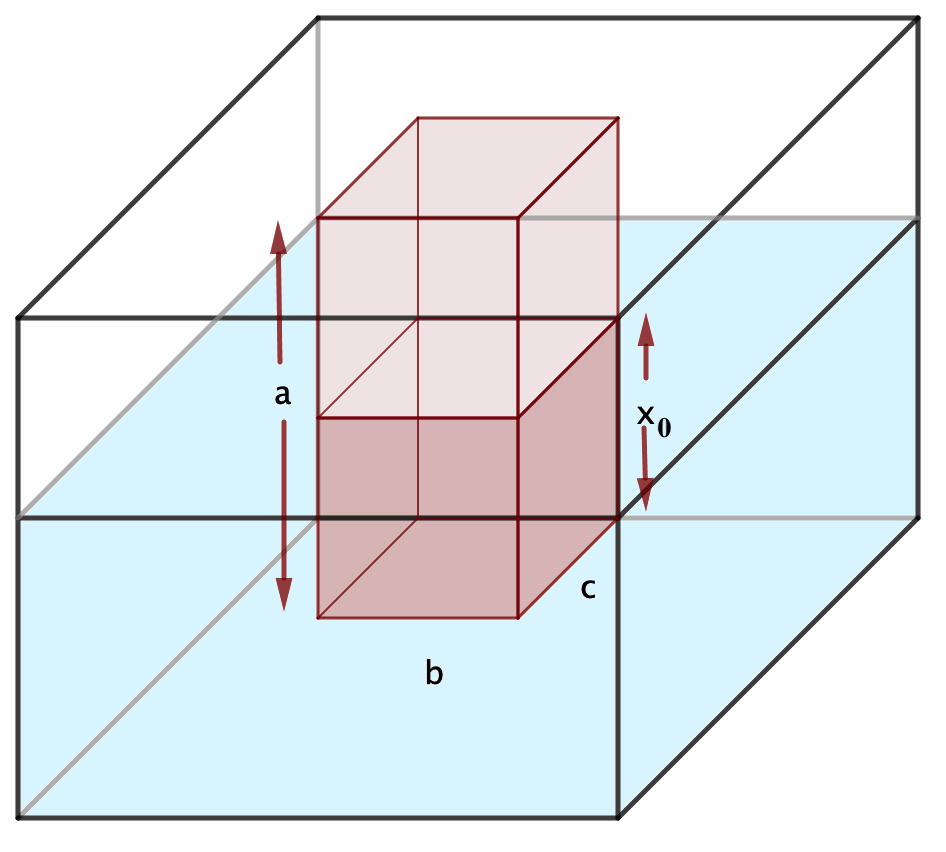
\includegraphics[width=.3\textwidth]{imagenes/imagenes21/T21IM08.png}
	\end{figure}	
\end{multicols}

$\cancel{\rho a g}-\cancel{\rho_0x_0g}-\rho_0xg=\rho a \ddot{x} \quad \to \quad \ddot{x}+\dfrac{\rho_o g}{\rho a}x=0\,\quad$ ec. MAS

Luego $\quad \omega^2=\dfrac{\rho_o g}{\rho a} \ \to \ \ T=2\pi \sqrt{\dfrac{\rho a}{\rho_0 g}}$

\vspace{5mm}%******************************
\begin{prob}
Un disco sólido de radio $R$ puede colgarse de un eje horizontal a una distancia $h$ de su centro.	Encontrar la posición a que hay que colgar el disco para la cual el periodo es máximo. 
\end{prob}
\begin{multicols}{2}
$T_{pend.\ compto.}=2\pi \sqrt{\dfrac{I}{mgh}}$

Th. Steiner: $I=I_0+mh^2=\dfrac 1 2 m R^2+mh^2$

$T=2\pi \sqrt{\dfrac{\dfrac {R^2}{2}+h^2}{gh}}=T(h)$

Para buscar el máximo, derivamos
\begin{figure}[H]
		\centering
		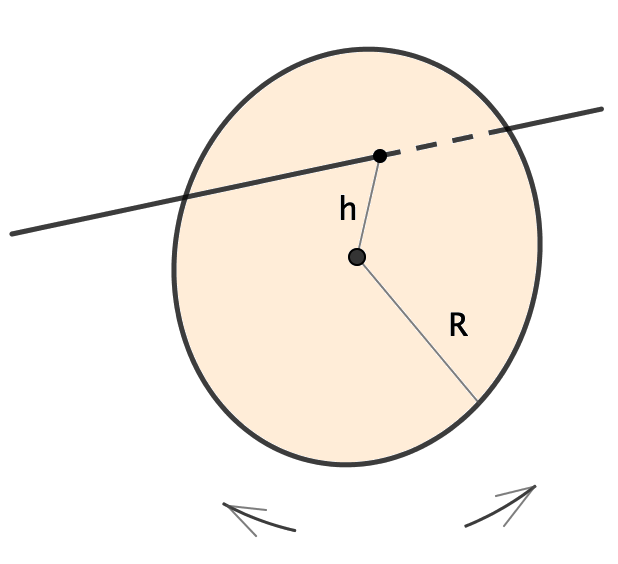
\includegraphics[width=.3\textwidth]{imagenes/imagenes21/T21IM09.png}
	\end{figure}	
\end{multicols}
$\displaystyle \dv{T}{h}=
\dfrac
{2\pi}
{2 \sqrt{ \dfrac{\dfrac {R^2}{2}+h^2}{gh}} } 
\dfrac{2gh^2-g \left( \dfrac{R^2}{2} + h^2 \right) } {g^2R^2} \ = \ 0 \leftrightarrow\ $ numerador es cer0.

$2\cancel{g}h^2-\cancel{g}\dfrac{R^2}{2}-\cancel{g}h^2=0 \ \to \ h_{min}=\dfrac{R}{\sqrt{2}}\quad $ Para esa $h_{min} \ \to \ T_{min}=2\pi \sqrt{\dfrac{\sqrt{2}R}{g}}$

$T(R)=\sqrt{\dfrac{3R}{2g}}; \quad T(0)\to \infty$, no oscila.

\vspace{5mm}%******************************
\begin{prob}
Una aro circular de $0.61\ \mathrm{m}$ de radio y $3.63\ \mathrm{kg}$ de masa se cuelga de un clavo horizontal. ?`Cuál es el periodo de oscilación para un movimiento de pequeña amplitud? ?`Cuál sería la longitud de un péndulo simple equivalente?	
\end{prob}

Suponemos que el aro gira colgado de un punto de su superficie.

$I=I_0+mh^2=2mR^2\quad (h=R); \qquad  T=2\pi \sqrt{\dfrac{I}{hmg}}=2\pi \sqrt{\dfrac{2R}{g}}=2.22\ \mathrm{s}$

$T=T_{pen.\ simple}=2\pi \sqrt{\dfrac l g} \quad \to \quad l=2R=1.22\ \mathrm{m}$
\vspace{5mm}%******************************
\begin{prob}
Un péndulo de torsión está constituido por un bloque de madera de $8\ \mathrm{cm}	\times 12 \ \mathrm{cm}	\times 3 \ \mathrm{cm}$ con masa de $0.3\ \mathrm{Kg}$. Al suspenderlo con un alambre con el lado más corto en posición vertical se mide el periodo de oscilación, resultando ser de $2.4\ \mathrm{s}$. ?`Cuál es la constante de torsión del alambre?
\end{prob}

$T=2\pi \sqrt{\dfrac I k};\quad I=\dfrac 1 {12} m (a^2+b^2); \quad k=4\pi^2 \dfrac {I}{T^2}=3.56\times 10^{-3} \ \mathrm{N \ m}$

\vspace{5mm}%******************************
\begin{prob}
\begin{multicols}{2}.

Dos resortes están unidos y conectados como muestra la figura a una masa $m$. Si los resortes, separadamente, tienen constantes $k_1$ y $k_2$, averiguar el periodo de oscilación del sistema.
\begin{figure}[H]
		\centering
		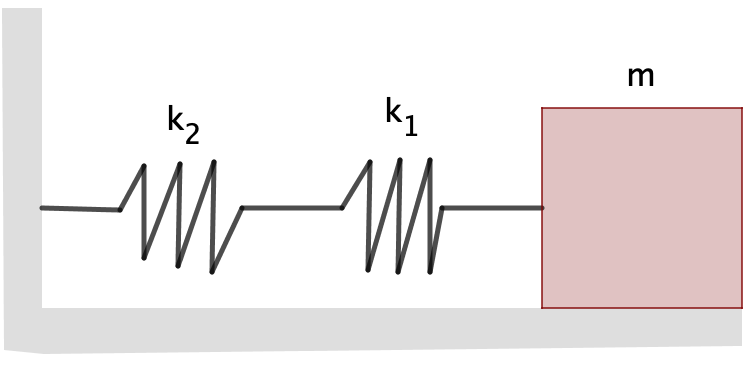
\includegraphics[width=.4\textwidth]{imagenes/imagenes21/T21IM10.png}
	\end{figure}	
\end{multicols}	
\end{prob}

$x=x_1+x_2 \begin{cases}
 F=-k_1x_1 \\
 F=-k_2x_2	
 \end{cases}
 k_ax_1=k_2x_2 \begin{cases}
 x_1=-\dfrac{m}{k_1}\ddot{x} \\  x_2=-\dfrac{m}{k_2}\ddot{x}	
 \end{cases}$

Sumando: $\ x_1+x_2 =\ x=-\left( \dfrac {m}{k_1} + \dfrac{m}{k_2} \right) \ddot{x} \quad \to \quad \ddot{x}+\dfrac {1}{\dfrac {m}{k_1} + \dfrac{m}{k_2}} \ x = 0$

$\omega^2 = \dfrac {1}{\dfrac {m}{k_1} + \dfrac{m}{k_2}} \quad \to \quad T=2\pi \sqrt{\dfrac{m}{k_1}+\dfrac{m}{k_2}}$ 

\vspace{5mm}%******************************
\begin{prob}.

\begin{multicols}{2}
Averígüese el periodo de oscilación del sistema de la figura cuando la masa $m$ y los resortes $K_1$ y $k_2$ están unidos como se indica.
\begin{figure}[H]
		\centering
		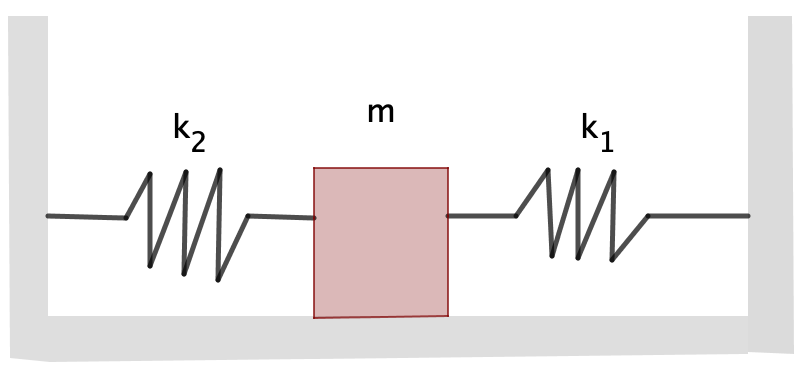
\includegraphics[width=.4\textwidth]{imagenes/imagenes21/T21IM13.png}
	\end{figure}	
\end{multicols}
\end{prob}

Para un pequeño desplazamiento $x$ de la masa $m$ hacia la derecha, el muelle $k_1$ se comprime y ejercerá fuerza hacia la izquierda, el muelle $k_2$ se estira y la fuerza también será hacia la izquierda. Ambas en el mismo sentido.

$F=-k_1x-k_2x=m\ddot{x} \ \to \ \ddot{x}+\dfrac{k_1çk_2}{m}x=0 \ \to \ \omega=\dfrac{k_1+k_2}{m} \ \to $

$ T=2\pi \sqrt{\dfrac{m}{k_1+k_2}}$

\begin{prob}
La escala de una balanza de resorte lee desde $0$ hasta $14.5\ \mathrm{kg}$ y tiene $10\ \mathrm{cm}$ de largo. Se sabe que un paquete colgado de la balanza oscila verticalmente con una frecuencia de $2.0$ oscilaciones por segundo	. ?`Cuánto pesa el paquete?
\end{prob}

$m=14.5\ \mathrm{kg}$; $\ x=0.1\ \mathrm{m}$; $\ T=\dfrac 1 2= 0.5 \ \mathrm{s}$

$F=-kx=mg \to k=\dfrac{mg}{x}$

$mg-kx=m\ddot{x} \to \ddot{x}+\dfrac{k}{m}x=g\ \textcolor{gris}{(cte)} \quad \omega^2=\dfrac k m \ \to \dfrac{4\pi^2}{T^2}=\dfrac k m \ \to \ m=k\dfrac{T^2}{4\pi^2} = 7.8\ \mathrm{kg}$

\begin{prob}
Un péndulo	simple tiene un perido de $2$ segundos y una amplitu de $2^o$. Después de $10$ oscilaciones completas su amplitud se ha reducido a $1.5^o$, encontrar la constante de amortiguamiento.
\end{prob}

$\theta_0=2^o;\ t=10 T \to \theta =1.5^o$

Movimiento amortiguado: 

$ \theta=\theta_0 e^{-\gamma t}\cos (\omega t + \alpha) \ \to \ \theta(t)=\theta_0 e^{-\gamma t} \ \to \theta=\theta_o e^{-\gamma 10 T}$

$\gamma=\dfrac {1}{10T} \ln \dfrac {\theta}{\theta_0}=0.014 \ \mathrm{s}^{-1}$







\newpage
\begin{myblock}{Frentes de onda y rayos}
	\begin{figure}[H]
		\centering
		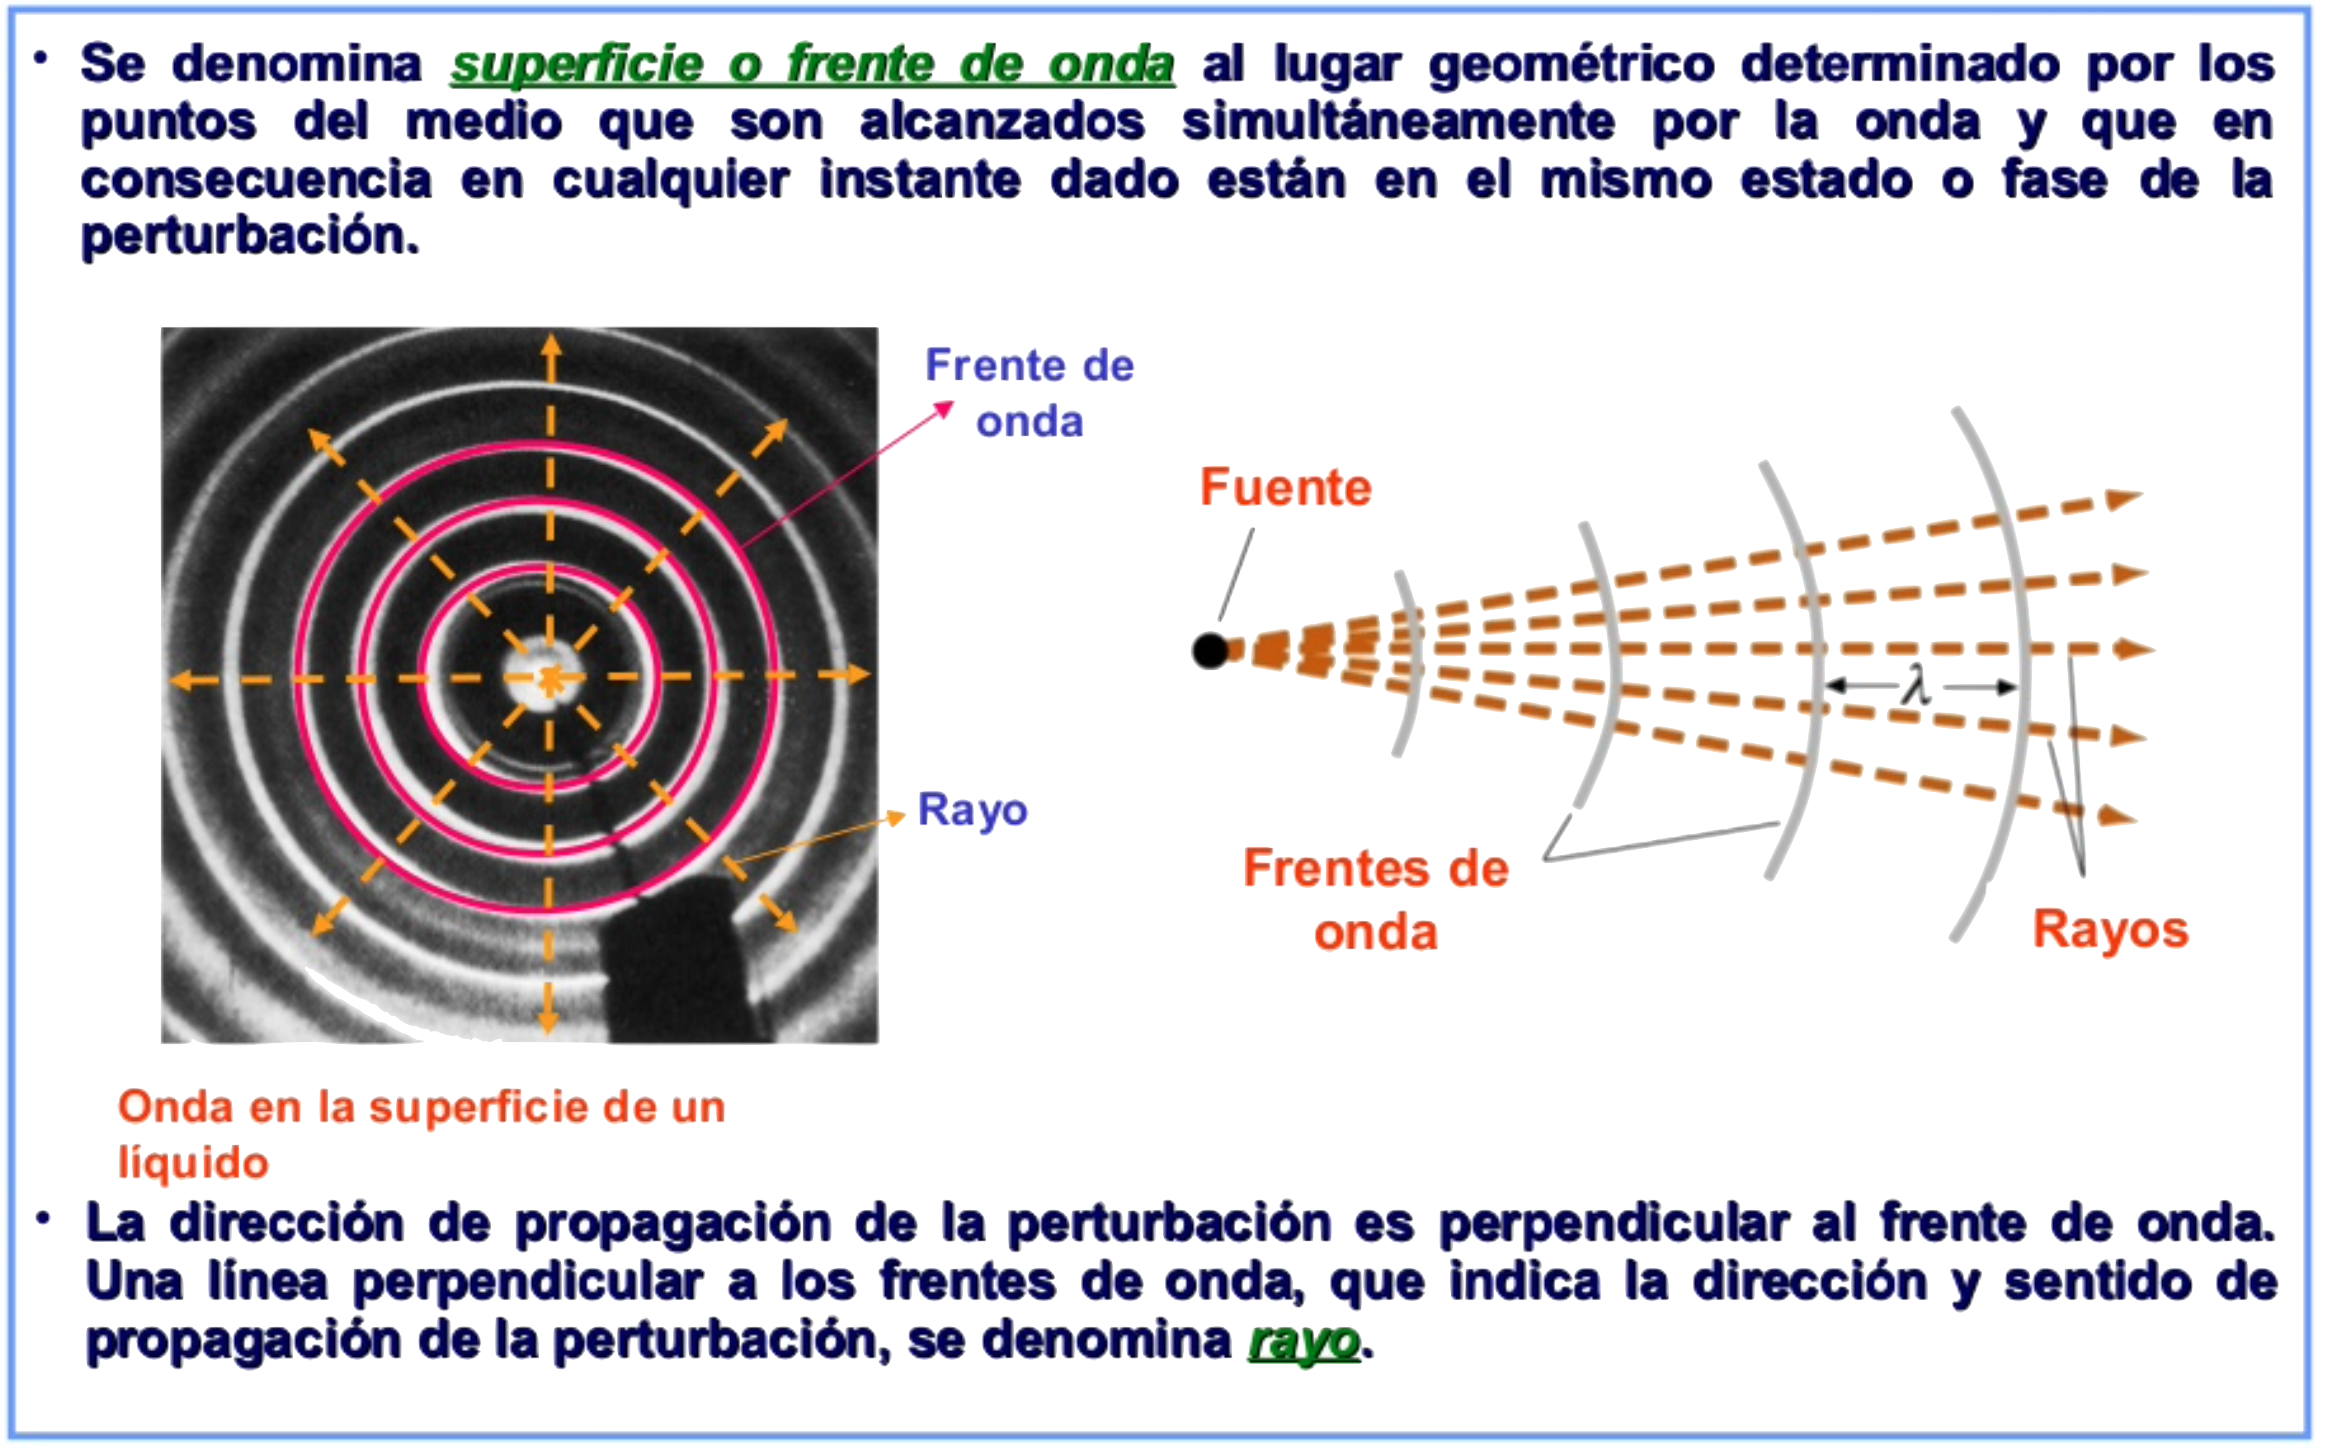
\includegraphics[width=1\textwidth]{imagenes/imagenes21/T21IM11.png}
	\end{figure}
	\begin{figure}[H]
		\centering
		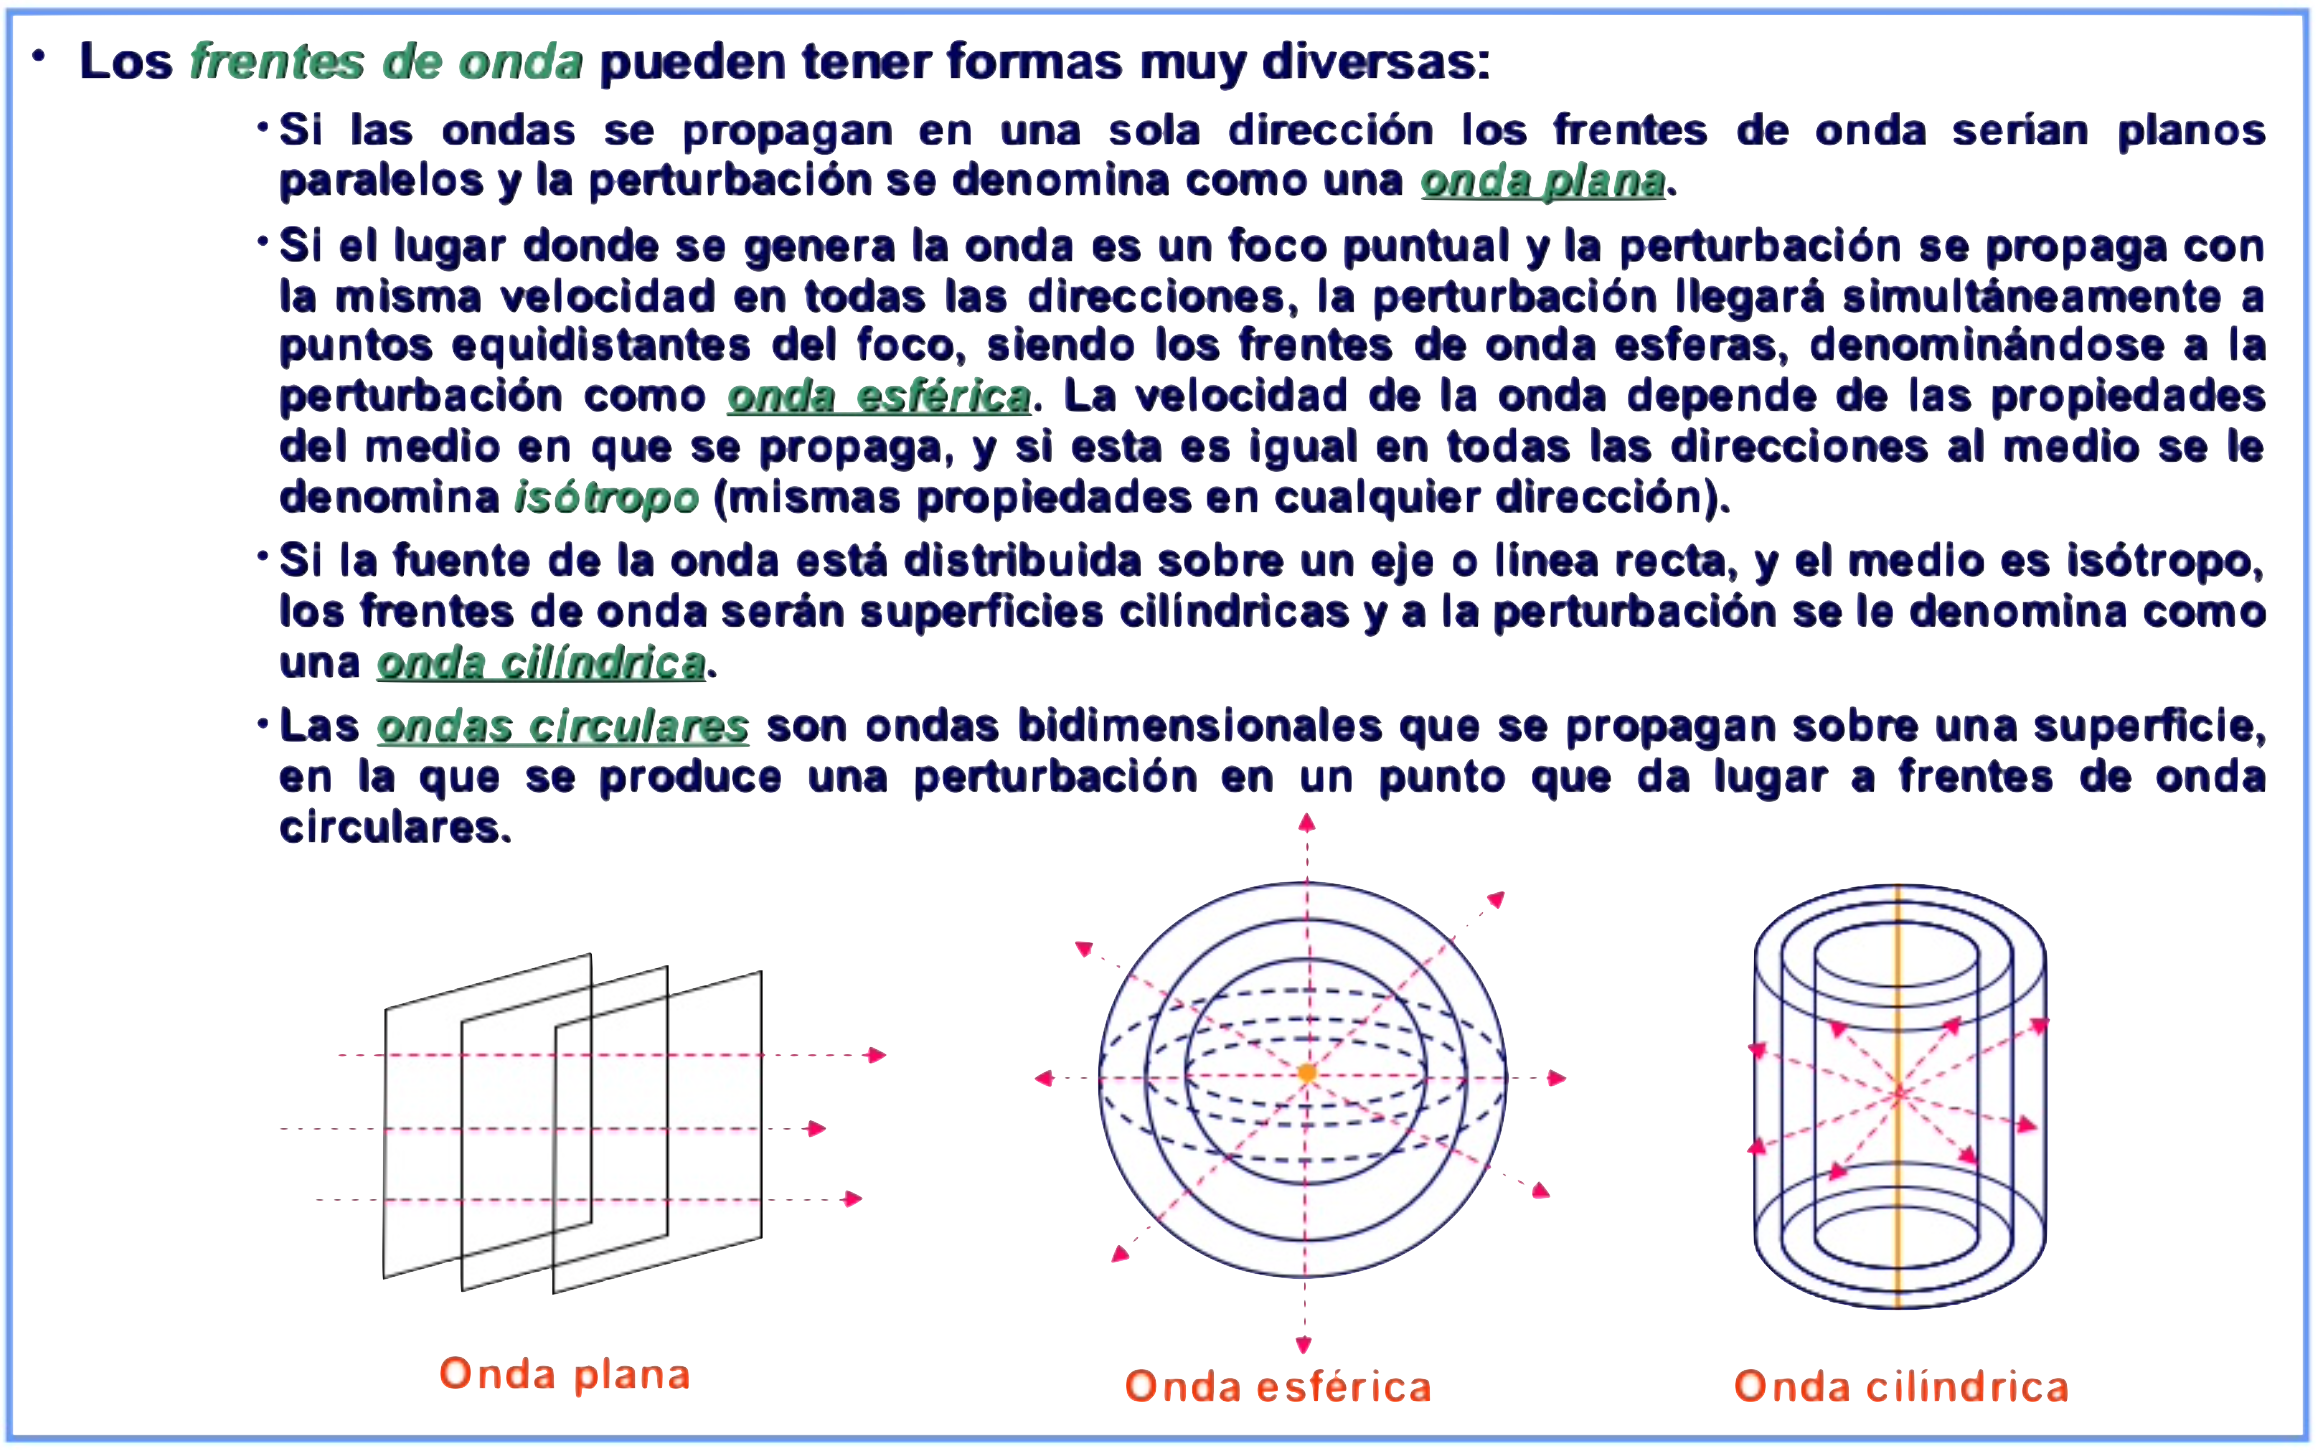
\includegraphics[width=1\textwidth]{imagenes/imagenes21/T21IM12.png}
	\end{figure}
\end{myblock}



